

\part{Language}

%
% Getting Started
%
\chapter{Getting Started}

\section{A Few Comments on Comments}

In the primer, you were briefly introduce to the concept of comments.  A comment is a section of the script that you can tell the interpreter to ignore.  This way you can write yourself, or others that are reading the script, useful notes. I wanted to cover comments first because they are both very simple and very useful.

Unlike nearly every other language, there are four types of comments in \SSquared.  Actually there are two types with two variations each.  All types are treated exactly the same by the interpreter, that is, they are completely ignored.  So why make a bunch of a different comment types?  Because \SSquared\ is meant to be read by humans, not just the person writing the script, but other humans too.  In fact, as far as the interpreter is concerned, all the comment types are the same.  However each comment does have an implicit purpose and is useful for writing a more readable script.

First I will list the syntax of each comment, then I will explain what they are used for.

\begin{SSCodeBox}
\SSCodeNumber{1} \\
\sciteg{// This is utility line comment}
\scitea{} \\
\scitea{} \\
\scitek{/* } \\
\scitek{This is a utility} \\
\scitek{block comment} \\
\scitek{*/}
\scitea{} \\
\scitea{} \\
\SSCodeNumber{2} \\
\sciteh{/$>$ This is a scene line comment}
\scitea{} \\
\scitea{} \\
\scitej{/. } \\
\scitej{This is a scene} \\
\scitej{block comment} \\
\scitej{./}
\scitea{} \\
\end{SSCodeBox}

\SSCodeNumber{1} These are utility comments.  They are used in much the same way as comments in other programming languages.  That is, they are used to make notes about something related to the actual script.  For example, to remind yourself of something that needs to be done.

\begin{SSCodeBox}
\scitel{Husband: TheGood}
\scitea{\{} \\
\sciteb{\'{}No way honey! You look fantastic!\'{}}
\scitea{;} \\
\scitea{\hspace*{4em}} \\
\scitea{\hspace*{4em}}
\sciteg{//TODO: Add a proper response for Wife.} \\
\scited{\hspace*{4em}next} 
\scitea{=}
\scited{end}
\scitea{;} \\
\scitea{\}} \\
\end{SSCodeBox}


The line comment form instructs the interpreter to ignore everything after \SSCode{//} up till a new line.  The block form of this comment causes the interpreter to ignore everything between \SSCode{/*} and \SSCode{*/}.  This is useful for larger comments.  They are also quite handy for ``commenting out'' large sections of code that you want to temporarily disable.

\begin{SSCodeBox}
\sciteg{// On second thought, I don't think we should have this option}
\scitea{} \\
\scitea{} \\
\scitek{/*} \\
\scitek{Husband: TheBad\{} \\
\scitek{\hspace*{4em}\'{}A little bit fat?{\hspace*{1em}} I think that's a little} \\
\scitek{\hspace*{4em}bit of an understatement\'{};} \\
\scitek{\}} \\
\scitek{*/}
\end{SSCodeBox}

If you a Java or C/C++ programmer you will quickly notice that utility comments are exactly the same as comments in these languages as well as several others.  All things being equal, I tried to choose syntax that would be familiar to those with previous programming experience.

\SSCodeNumber{2} The second type of comment we will discuss is the scene comment. The scene comment is used to describe what is happening in the scene.  I mentioned earlier that \SSquared\ scripts are meant as a blueprint for a team to work off of the create a game.  Scene comments give other people reading the script the information they need to create the scene.

\begin{SSCodeBox}
\scitea{} \\
\scitej{/.} \\
\scitej{Husband is a sitting alone reading\\ a newspaper and enjoying a sandwich.} \\
\scitej{Wife enters wearing an unflattering\\ blouse with the tag still attached.} \\
\scitej{./}
\scitea{} \\
\scitea{} \\
\scitel{Wife: TheQuestion}
\scitea{\{} \\
\sciteb{\'{}Does this blouse make me look a little bit fat?\'{}}
\scitea{;} \\
\scitea{\hspace*{4em}} \\
\scitea{\hspace*{4em}}
\scited{next}
\scitea{=} \\
\scitea{\hspace*{4em}Husband: TheGood,} \\
\scitea{\hspace*{4em}Husband: TheBad,} \\
\scitea{\hspace*{4em}Husband: TheUgly;} \\
\scitea{\}}
\end{SSCodeBox}

The syntax is similar to utility comments.  Everything after \SSCode{/>} is ignored up till the next line, and in the block form, everything between \SSCode{/.} and \SSCode{./} is ignored.

The difference between utility comments and scene comments are of course by convention, the interpreter doesn't care how you use them.


\section{Naming Rules}

Remember in the primer when I told you to pay special attention to how we declare characters?  That was because variables, lists, players, and characters are all declared using the same syntax.

\begin{SSCodeBox}
\scited{character} 
\scitea{Alfred};
\end{SSCodeBox}

Variables and Lists will be covered a little later but it is important to talk about identifier names first.  There are limits to what you can named objects. Valid identifier names can be any length\footnote{Theoretically.  Your computer still has a limited memory supply.} and can contain any combination of letters, numbers, or underscores ("\_").  

There two exceptions to those rules. First, you cannot use a name that is already in use.  There are some special variables that are already in existence before you do anything.  We will talk about those later on.  The second exception is that a names can't start with a digit.  The rationale being that identifiers starting with a digit can create ambiguous situations in which \SSquared\ can't tell if it is really dealing with an identifier or with a number.  Besides that, how you name variables is mostly up to you.  Try to pick names that accurately describe what that variables is for.

\begin{SSCodeBox}
\scited{character}
\scitea{ Charlies\_wifes\_former\_college\_roomates\_uncle;} \\
\scited{character}
\scitea{ UncleJoe;}
\end{SSCodeBox}

Any of these are valid, just pick a naming convention that works for you and stick with it.

\begin{SSCodeBox}
 \sciteg{// This will not work!} \\
 \scited{character}
 \scitea{ 3Jane;}
\end{SSCodeBox}

This however will not work, but it shouldn't be hard to get around this limitation with a little creativity.

\begin{SSCodeBox}
 \scited{character}
 \scitea{ \_3Jane;} \\
 \scited{character}
 \scitea{ ThreeJane;} \\
\end{SSCodeBox}




%
% Types
%
\chapter{Types}

\section{Overview}

\SSquared\ is what is referred to in programmer jargon as \emph{weakly typed} (as opposed to \emph{strongly typed}.  Weak typings mean that \SSquared\ will convert between the types automatically and fluidly.  You should rarely have to worry about what type something is.  If I did a good job writing \SSquared\ then you should be able to use it without even knowing what a type is.  Nevertheless I need to cover types anyway.  

\subsection{Terminology}
I'm going to be mentioning variables and literals a lot coming up, so it is important that I explain what they are and what the difference is.  A variable is a named object that hold a value.  Variables get covered in depth latter on.  Literals on the other hand are values that a literally written out.  If I wrote \SSCode{20} that would be a literal.  If I had a variable named \SSCode{MyAge} that held the value ``20'', that would be a variables.  The interpreter mostly doesn't care which is which.  It only knows that it can't modify the values of literals and it can modify the values of variables.

\subsection{Numbers}
The three central types are numbers, strings, and booleans.  Numbers are of course just numbers.  In \SSquared\ numbers are really variable precision floating-point numbers, which just means that you can use very small and very large numbers without having to worry about loosing precision (like you do with calculators).  

Writing number literals is pretty straightforward:

\begin{SSCodeBox}
\scitec{42} \\
\scitec{3.1415926535897932384626433832795028841971} \\
\scitec{-1000} \\
\scitec{0}
\end{SSCodeBox}

A number must start with a digit and have one or zero decimal points.   You may also put a minus sign in front of a number literal to make it negative.

\subsection{Strings}
Strings are just text of any kind.  Just put (almost) whatever you want between two quotation marks and you have yourself a string.   In normal use of \SSquared\ (i.e. writing scripts for games) you will make much more use of strings than anything else.

\begin{SSCodeBox}
\sciteb{"This is a string."}
\end{SSCodeBox}

In the primer I had you using backticks instead of quotation marks.  There is a reason for that that will be explained in the chapter or blocks.  Just bear with me for now.  There are a few special tricks with strings in \SSquared\.  First of all, if you put two strings next to each other, regardless of how much whitespace is between them, the interpreter will read that as a single string.  I refer to this as string stacking.

\begin{SSCodeBox}
\sciteb{"This "\\"is one string, "  "as far as the interpreter is concerned."}
\end{SSCodeBox}

One other odd thing about strings in \SSquared\ is that whitespace is edited out.  In this way \SSquared\ is similar to HTML or \LaTeX{}.  Consider this paragraph, in which the writer used tabs, spaces, and newlines to apply ``artificial'' formatting:

\begin{SSCodeBox}
\scited{print}
\scitea{ }
\sciteb{"The year was 2081, and everybody was} \\
\sciteb{{\hspace*{1em}}{\hspace*{1em}}{\hspace*{1em}}{\hspace*{1em}}{\hspace*{1em}} finally equal.{\hspace*{1em}} They weren't only} \\
\sciteb{{\hspace*{1em}}{\hspace*{1em}}{\hspace*{1em}}{\hspace*{1em}}{\hspace*{1em}} equal before God and the law.{\hspace*{1em}} They} \\
\sciteb{{\hspace*{1em}}{\hspace*{1em}}{\hspace*{1em}}{\hspace*{1em}}{\hspace*{1em}} were equal in every which way."}
\scitea{;}
\end{SSCodeBox}

If you executed that the output will be something like this:

\begin{SSCodeBox}
\sciteb{The year was 2081, and everybody was finally equal.  They weren't only equal before God and the law.  They were equal in every which way.}
\end{SSCodeBox}

This is because \SSquared\ will edit out any newlines and extra spaces or tabs at the beginning of a line.  The rationale for this is to allow writers to write line of dialogue however they want without it affecting what gets shown on screen.  This can be overridden however.

The final strange thing that strings do is interpret any character after a backslash literally.  This way, you can put a backslash at the end of a line, and it will keep that newline instead of editing it out.

\begin{SSCodeBox}
\scited{print}
\scitea{ } \\
\sciteb{"Break, break, break,{\textbackslash}} \\
\sciteb{On thy cold gray stones, O Sea!{\textbackslash}} \\
\sciteb{And I would that my tongue could utter{\textbackslash}} \\
\sciteb{The thoughts that arise in me."}
\scitea{;}
\end{SSCodeBox}

\noindent{}This behavior is also useful if you want to include quotation marks inside a string.

\begin{SSCodeBox}
\sciteb{"\textbackslash"No, I didn't,\textbackslash" said Alice: \textbackslash"I don't think it's at all a pity. I said 'What for?'\textbackslash""}
\end{SSCodeBox}

\noindent{}Alice's little quip gets printed properly this way.

\begin{SSCodeBox}
\sciteb{"No, I didn't," said Alice: "I don't think it's at all a pity. I said 'What for?'"}
\end{SSCodeBox}


\subsection{Booleans}

Booleans are simply true or false values.  ``What good are true/false values?'' you ask.  For the results of comparison operators mainly.  Boolean literals take two forms of course:

\begin{SSCodeBox}
\scited{true} \\
\scited{false}
\end{SSCodeBox}

\subsection{Transliteration}

\SSquared\ will for the most part convert between these types seamlessly, but there are a few special cases that it pays to be aware of.  First off, any number (even zero) is considered ``true'' in the boolean context.  The only number that is considered false is the special NaN (``Not-A-Number'') value which is the result of bad math operations (such as dividing by zero).  With strings, empty strings are considered false, all other strings are considered true.


\section{Variables}

\subsection{Overview}

With types and literals pretty well explained we can move onto variables.  Variables are simply named objects which hold a value.  Unlike some other high level languages, variables must be declared in \SSquared{}.  The syntax for declaring variables is pretty simple though.  It is merely the \SSCode{var} keyword followed by a name. 

\begin{SSCodeBox}
\scited{var}
\scitea{ Foo;}
\end{SSCodeBox}

\noindent{}Naturally, all the usual naming restrictions apply.  ``Foo'' can now be used in expression however you like.

\begin{SSCodeBox}
\scitea{Foo = }
\sciteb{"Bar"}
\scitea{;}
\end{SSCodeBox}

\subsection{Magic Variables}

Variables have some special built in properties that you can modify.  Indeed some of these are common to all objects in \SSquared{}, but I may as well cover them here.  

One that is unique to variables is the \SSCode{precision} property.  The precision property gives a simple method for increasing the precision of the numbers stored in an individual variable.  Usually you won't have to mess with this, but it is useful sometimes if you want to perform some ridiculous calculation.  These properties are accessed using the scope resolution operator.

\begin{SSCodeBox}
\scitea{Foo: precision = }
\scitec{512}
\scitea{;}
\end{SSCodeBox}

The number assigned to precision gives the number of bits of precision.  There isn't a simple way to translate between bits and digits so you may have to just use trial and error.  By default the precision is set pretty high (in the current version, 256), but there is also a way to change the default precision of variables.  This gets covered in the section covering ``LangOpts'' in the last chapter.

It is important to note that the precision variable is magic.  What I mean by that, is that it behaves like a normal variables in every way on the outside, but when you assign a number to it, but in background it changes the precision of the variable.  Magic variables are a little like the pastors daughter who behaves perfectly when in respectable company but snorts coke with her friends when her parents aren't around.

There are also a couple properties which are common to every object in \SSquared{}.  One is the \SSCode{name} variable, which simply holds the name of the variable.  However, currently you cannot assign to the name variable (i.e. you can't change the name of a variable after you created it).  So (provided you followed instruction and declared the Foo variable) feeding this into the interpreter:

\begin{SSCodeBox}
\scited{print}
\scitea{ Foo: name;}
\end{SSCodeBox}

\noindent{}Will print out:

\begin{SSCodeBox}
\sciteb{Foo}
\end{SSCodeBox}

One last magic variable I should cover is just a variation of the name variable.  That is the \SSCode{fullname} variable, which spits out the name of the variable along with all its parents and grand-parents.

\begin{SSCodeBox}
\scited{print}
\scitea{ Foo: fullname;}
\end{SSCodeBox}

\noindent{}That code, depending on where Foo was declared, and what the name of the file is, will print out something like this:

\begin{SSCodeBox}
\sciteb{:test\_ssconv:Foo}
\end{SSCodeBox}

This may not make perfect sense until we explore the language more, so I'll just leave it at that.

\subsection{Constants}

There are few constants which are variables which are predefined by the language and cannot be modified.  They represent certain special values that are often useful to reference.

\BeginSSTable{|c|c|}{h}
\textbf{Constant} & \textbf{Description} \\
endl & Newline \\
\_INF\_ & Infinity \\
\_NEGINF\_ & Negative Infinity \\
\_NAN\_ * Not-A-Number \\
\EndSSTable{Language Constants}

The \SSCode{endl} constant is a conveniant way to inserting or printing a newline without having to have a backslash followed by an actual newline.  The others are more mathematical, but do have their uses, such as checking for division by zero or other bad operations.



\section{Lists}

\subsection{List Literals}

Lists are a compound made up of zero or more individual variables.  The are ordered and numbered.  And can be grown, shrunk, sorted, elements can be inserted, or removed.  

List literals are simple two or more variables or literals separated by commas.

\begin{SSCodeBox}
\scitec{1}
\scitea{, }
\scitec{2}
\scitea{, }
\scitec{3}\\
\sciteb{"a"}
\scitea{, }
\sciteb{"b"}
\scitea{, }
\sciteb{"c"}\\
\scitea{Alabama, Alaska, Arizona}
\end{SSCodeBox}

Those ones are all valid lists (the last one only is if \SSCode{Alabama}, \SSCode{Alaska}, and \SSCode{Arizona} are all declared variables).  You can mix variables and literals of course.  There is one special case list literal: the empty list literal.  The empty list literal is simply parenthesis with nothing between this: \SSCode{()}.  This has one very special use when it comes to calling function without passing any parameters. But right now you can use it to clear lists or check if their empty.

\subsection{Declaring Lists}

Declaring lists is pretty straightforward.  The syntax is just like declaring variable, but with the \SSCode{list} keyword.

\begin{SSCodeBox}
\scited{list}
\scitea{ ItalianPainters = } \\
\scitea{\hspace*{4em}}
\sciteb{"Leonardo"}
\scitea{,} \\
\scitea{\hspace*{4em}}
\sciteb{"Michelangelo"}
\scitea{,} \\
\scitea{\hspace*{4em}}
\sciteb{"Donatello"}
\scitea{,} \\
\scitea{\hspace*{4em}}
\sciteb{"Raphael"}
\scitea{;}
\end{SSCodeBox}

\subsection{Simple List Operations}

\noindent{}All the standard things that you would expect to able to with lists will work.

\begin{SSCodeBox}
\scited{list}
\scitea{ TeenageMutantNinjaTurtles = ItalianPainters;} \\
\scited{print}
\scitea{ TeenageMutantNinjaTurtles;} \\
\sciteg{//That will print "LeonardoMichelangeloDonatelloRaphael"}
\end{SSCodeBox}

Accessing individual object inside a list uses the brackets (``[ ]'') with an index.  Be careful though.  The first element in the list is element zero not element one.  So the second element in a list has an index of one.  It is a pretty common mistake with beginner programmers to forget this and get ``off-by-one'' bugs in their programs.

\begin{SSCodeBox}
\scited{print}
\scitea{ TeenageMutantNinjaTurtles[}
\scitec{0}
\scitea{];} \\
\sciteg{//Leonardo will be printed}
\scitea{} \\
\scited{print}
\scitea{ TeenageMutantNinjaTurtles[}
\scitec{3}
\scitea{];} \\
\sciteg{//Raphael will be printed, last but not least of the turtles.}
\end{SSCodeBox}

The default behavior of lists in \SSquared\ is to spring new elements into existence when you access an index doesn't have anything stores in it.
If you accidentally try to access Raphael by using an index of four, nothing catastrophic will happen because new element will be created at the end of the list.  Try it.

\begin{SSCodeBox}
\scited{print}
\scitea{ TeenageMutantNinjaTurtles[}
\scitec{4}
\scitea{];}
\end{SSCodeBox}

That will simply print \SSCode{false}, which is the default value for uninitialized variables.  We can go ahead and assign something to that element though.

\begin{SSCodeBox}
\sciteg{//An honorary Turtle.}
\scitea{} \\
\scitea{TeenageMutantNinjaTurtles[}
\scitec{4}
\scitea{] = }
\sciteb{"Casey Jones"}
\scitea{;}
\end{SSCodeBox}

If you access an element even farther ahead, say element 44, the list will just make the list long enough by adding forty new elements onto the end.

\subsection{Insertion and Removal}

There are special operators used to insert and removal elements from a list.  The insertion operator is like list access operator but with a plus before it.

\begin{SSCodeBox}
\scitea{TeenageMutantNinjaTurtles+[}
\scitec{1}
\scitea{] = }
\sciteb{"Splinter"}
\scitea{;}
\end{SSCodeBox}

Notice the plug sign.  Printing the new list will give us ``LeonardoSplinterMichelangeloDonatelloRaphaelCaseyJones.''  Quite a mouth full.  You can probably guess what the removal operator looks like.  Lets remove Splinter, since he's kind of a jerk.

\begin{SSCodeBox}
\scitea{TeenageMutantNinjaTurtles-[}
\scitec{1}
\scitea{];}
\end{SSCodeBox}

No the the second element (remember, the count starts at zero) has been remove and the elements to the right have slid back to fill in the gap.  In the same way that the insertion operator evaluates to be the element inserted, the removal operator evaluates to be the element removed.

\begin{SSCodeBox}
\scited{print}
\scitea{ TeenageMutantNinjaTurtles-[}
\scitec{1}
\scitea{];}
\end{SSCodeBox}

So if instead we put print before it, it will remove Splinter from the list and then print ``Splinter.''  But splinter won't be in the list any longer.  Good, he's a killjoy.

\subsection{Compound Assignment}

Compound assignment is a cool little trick that you might come across or even find useful.  Consider our experiments with lists in the previous paragraphs.  We can assign to list literals too, provided they are made up of modifiable variables.  Here's how it works.

\begin{SSCodeBox}
\scited{var}
\scitea{ BestLookingTurtle;} \\
\scited{var}
\scitea{ WhiniestTurtle;} \\
\scited{var}
\scitea{ SmartestTurtle;} \\
\scited{var}
\scitea{ LeastMatureTurtle;} \\
\scitea{} \\
\scitea{(BestLookingTurtle, WhiniestTurtle, } \\
\scitea{SmartestTurtle, LeastMatureTurtle) = TeenageMutantNinjaTurtles;} \\
\scitea{} \\
\scited{print}
\scitea{ SmartestTurtle;}
\end{SSCodeBox}

That will print ``Donatello'' who everyone knows is an intellectual giant compared to his pizza hogging cohorts.  You can also just assign from one literal to another.

\begin{SSCodeBox}
\scitea{Afghanistan\_Capital,} \\
\scitea{Albania\_Capital,} \\
\scitea{Algeria\_Capital = }
\sciteb{"Kabul"}
\scitea{, }
\sciteb{"Tirana"}
\scitea{, }
\sciteb{"Algiers"}
\scitea{;}
\end{SSCodeBox}

\subsection{List Magic Variables and Operators}

There are some very useful things built into every list.  The first is the \SSCode{size} magic variable.  The size variable, as you can probably guess, provides a simple interface for controlling the size of list.

\begin{SSCodeBox}
\scited{print}
\scitea{ ItalianPainters:size;}
\end{SSCodeBox}

That should print ``4'', since we currently have four Italian painters listed.  If we want fewer Italian painters we can modify the size variable.

\begin{SSCodeBox}
\scitea{ItalianPainters:size = }
\scitec{2}
\scitea{;} \\
\scited{print}
\scitea{ ItalianPainters;}
\end{SSCodeBox}

That will now print just ``LeonardoMichelangelo''.  You can use the size variable in any other way that would use a variable.  You can set it to a higher value and the list will create elements to fill in.  I would increase the size, but the only Italian painters I know are the ones I learned from watching Teenage Mutant Ninja Turtles.

Now comes the really fun stuff.  I haven't covered operators in any detail but I'm going to introduce some here anyway.  Don't worry if you don't fully understand them, because you will.

Lists come with several operators built in that will modify the list is some way.  The first two are \SSCode{push} and \SSCode{pop}.  Push and Pop are like using the add and insert operators on the end of a list.  Let me demonstrate.  Lets say we have our intact list of four Italian painters.

\begin{SSCodeBox}
\scitea{ItalianPainters:}
\scited{push}
\scitea{ }
\sciteb{"Vincent Van Gogh"}
\scitea{;}
\end{SSCodeBox}

That adds Vincent Van Gogh to the end list.  The you also pass another list or list literal to the push operator and it will add every object from that list to the end of your original list.  Actually, Vincent Van Gogh is Dutch, so I guess we have to remove him.  We can employ pop for that.  Remember when I said the empty list literal ( \SSCode{()} ) has a special purpose?  Well pay attention.

\begin{SSCodeBox}
\scitea{ItalianPainters:}
\scited{pop}
\scitea{();}
\end{SSCodeBox}

Van Gogh is now removed from the list and we are back to our original four.  The pop operator doesn't take any arguments, but if we don't put something after it, \SSquared\ has know way to know if want to execute pop, or want to just refer to the pop operator in some way.  So we pass it an empty list as any argument.  This is the same syntax used to call functions with no arguments in many other languages, which is why I made the empty list literal \SSCode{()}.

The other two built in operators or \SSCode{remove} and \SSCode{removeall}.  If you give remove an argument it will remove the first occurrence of that operator

\subsection{Interpolation}

Keeping with the weak-typings, lists and variables are converted between each other pretty freely.  When lists get cast to variables, they will just squash all their elements together.  So \SSCode{(1, 2, 3)} converted to a variable, will look more like \SSCode{(123)}.  On the flip side, variable being converted to lists, will simply create a single element list.  That single element will be the value of the variable.

%
% Operators
%
\chapter{Operators}

\section{Terminology}
An operator is something that performs an operation.  There are really two type of operators in \SSquared{}.  Built-in binary operators, and unary operators.  Unary operators are also sometimes referred to as functions, because \SSquared\ tries not to make much of a distinction between the two.

An expression is anything that evaluates to something.  That is, anything the interpreter can read and get a value from, is an expression.  \emph{Anything} that produces a value is an expression.  For instance, \SSCode{2 + 2} is an expression, because it evaluates to be 4.  So is a just a plain variable name, because a variable name evaluates to the the value that it is currently holding.  So is just \SSCode{4}, because it evaluates to be 4.  That may sound more confusing than it is.

Usually expressions perform some kind of operation.  Expressions usually consist of operators performing operations on variables and literals.  Operators take many forms, including common math operators like \SSCode{+, -, *, /}.  There are also boolean operators such as \SSCode{and, or, not}.  All of these are covered in the next few sections.

\section{Binary Operators}

Binary operators, as you can tell from the name, perform an operation on two objects.  You are already familiar with many binary operators if you have taken grade school math\footnote{At least that's what I heard.  I still haven't passed.}  Simple math operations such as +, -, *, etc, are all binary operators, and are all in \SSquared{}.  But there are quite a few more.  Look at \textbf{Table 3.1} to see all of them.

\BeginSSTable{|c|c|}{h}
+ & Addition \\
- & Subtraction \\
/ & Division \\
$*$ & Multiplication \\
\verb=^= & Exponentiation \\
. & Concatenate \\
= & Assignment \\
+= & Add and Assign \\
-= & Subtract and Assign \\
/= & Divide and Assign \\
$*${}= & Multiply and Assign \\
\verb=^== & Exponentize and Assign \\
.= & Concatenate and Assign \\
== & Equal To \\
> & Greater Than \\
< & Less Than \\
>= & Greater Than or Equal To \\
<= & Less Than or Equal To \\
and & Logical And \\
or & Logical Or \\
\EndSSTable{Binary Operators}

There isn't anything unusual here to those who have used high level languages like Perl or Python.  To those knew to programming, don't worry, its pretty simple.  I'm going to give a quick rundown of all the binary operators in \SSquared{}, but if you prior programming experience and have seen these all before, you can skip this part, or you can go through it anyway, just for the pleasure of reading my charming and provocative prose.

The addition, subtraction, division, and multiplication (\SSCode{+, -, /, $*$} operators all operate just like in elementary school math.  They do not however change any of the original values though.

\begin{SSCodeBox}
\scited{var}
\scitea{ foo = }
\scitec{2}
\scitea{;} \\
\scitea{foo + }
\scitec{2}
\scitea{; }
\sciteg{//This adds 2 to foo and does nothing with the result}
\scitea{} \\
\scited{print}
\scitea{ foo; }
\sciteg{//prints 2}
\end{SSCodeBox}

Feel free to experiment with that.  To actually add two to foo and have the result stick, is where the various ``x-and-assign'' operators come in.

\begin{SSCodeBox}
\scited{var}
\scitea{ foo = }
\scitec{2}
\scitea{;} \\
\scitea{foo += }
\scitec{2}
\scitea{; }
\sciteg{//This adds 2 to foo and and the result is stored in foo}
\scitea{} \\
\scited{print}
\scitea{ foo; }
\sciteg{//prints 4}
\end{SSCodeBox}

This an equals sign after the other operator has the same effect of performing the operating and assigning it the variable.  

Before I move onto the comparison and boolean operators, there is one more exotic operator I have to cover: the concatenation operator.  The concatenation operator interprets two objects as strings and pushes them into one.

\begin{SSCodeBox}
\scited{print}
\scitea{ }
\scitec{1}
\scitea{ + }
\scitec{2}
\scitea{ + }
\scitec{3}
\scitea{;} \\
\sciteg{//Prints "6"}
\scitea{} \\
\scitea{} \\
\scited{print}
\scitea{ }
\scitec{1}
\scitea{ . }
\scitec{2}
\scitea{ . }
\scitec{3}
\scitea{;} \\
\sciteg{//Prints "123"}
\end{SSCodeBox}

Even though those are numbers, they are seamlessly converted to strings and stuck all together.  It should also be noted that the addition operator \SSCode{+} will behave like the concatenation operator if it can't figure out how to convert something to a number.

The comparison operators are different in that they always result a boolean result.  You can think of them as assertions, which the interpreter will then check and return true if the statement is true, and if the statement is false it will call you on your BS and return false.  These operators really do have a use, just wait until we get to Control Constructs chapter.

\begin{SSCodeBox}
\scited{print}
\scitea{ }
\sciteb{"pie"}
\scitea{ == }
\sciteb{"pie"}
\scitea{;} \\
\sciteg{//Prints "true"}
\scitea{} \\
\scitea{} \\
\scited{print}
\scitea{ }
\scitec{10}
\scitea{ $>$ }
\scitec{100}
\scitea{;} \\
\sciteg{//Prints "false"}
\scitea{} \\
\scitea{} \\
\scited{print}
\scitea{ }
\sciteb{"toast"}
\scitea{ $>$ }
\sciteb{"pie"}
\scitea{;} \\
\sciteg{//Prints "true"}
\end{SSCodeBox}

Lets me explain the last example, before pie fans start emailing me.  Many of the operators in \SSquared\ will desperately try to do something useful.  In the current version of \SSquared\ if you compare two strings that cannot be converted to numbers, the lengths of the strings will be compared.  It is not advisable to depend on this behavior however.  \SSquared\ is still a young language and this may very well change in future versions.

Notice also that the operator that tests for equality is \SSCode{==}.  That's two equals signs, not one.  One equals sign assigns a value two a variable, two equals signs tests for equality.  This is another common mistake made by many programmers, not just beginners either.

The last two binary operators, the logic operators, are unusual.  They too evaluate to boolean true/false results. But their arguments are also booleans.  The \SSCode{and} operator will evaluate to true if and only if \emph{both} its arguments evaluate to true, otherwise the result will be false.  The \SSCode{or} operator on the other hand will evaluate to true if either of its arguments are true, if both are false, then it will evaluate to false.  If this sounds confusing, I provided a little table.

\BeginSSTable{|c|c c|}{h}
     & true & false \\
\hline
true  & true & true \\
false & true & false \\
\EndSSTable{or}

\BeginSSTable{|c|c c|}{h}
     & true & false \\
\hline
true  & true & false \\
false & false & false \\
\EndSSTable{and}

Logical operators are mostly used in conjunction with comparison operators.

\begin{SSCodeBox}
\scited{pi}
\scitea{ == }
\sciteb{"pie"}
\scitea{ }
\scited{or}
\scitea{ }
\scited{pi}
\scitea{ == }
\scitec{3.1415}
\end{SSCodeBox}

There is one trick to the two boolean operators that makes them unique in \SSquared{}.  Boolean operators will short-circuit.  Short circuiting is when part of an expression isn't evaluated, because it doesn't have to be.  This arises from the fact that the \SSCode{and} operator will return false if either side of the expression is false, regardless of what the other side is.  The \SSCode{or} operator does just the opposite.  This allows us to ignore the other side of the expression in these cases.

This isn't something you will typically have to worry about, but in more advanced scripts in may create a bug if you aren't aware of it.  So once again for the record:  if whatever is to the left of an \SSCode{and} operator evaluates to be false, then it will immediately return false without bothering to evaluate the right side.  For the \SSCode{or} operator, if the left side evaluates and true, then it will return true and skip the right side.


\section{Unary Operators}

Unary operators perform an operation on on object.  As mentioned, in \SSquared\ they are mostly considered the same thing as functions.  If you've taken math high enough to know what functions are, than you have a good idea what \SSquared\ unary operators are like.  On important difference between the two is that users can create their own\footnote{Which is covered in the chapter on blocks.} unary operators.  Though in this section we just cover the semantics and the built-in unary operators.

Unary operators take just one argument.  Which is a single variable or a single list.  You have already seen a few unary operators, although you may not know it.  The \SSCode{var} and \SSCode{list} keywords are both unary operators, although they are somewhat unusual in that they take unused names as arguments instead of actual variables.

For now there are only two other unary operators that you need to know about.  The first is another logical operators like \SSCode{and} and \SSCode{or}: \SSCode{not}.  The \SSCode{not} operator simply reverses the boolean value it is given.

\begin{SSCodeBox}
\scited{print}
\scitea{ }
\scited{not}
\scitea{ false;}
\end{SSCodeBox}

That will print true.  If you do the same with true, it will print false.

The other unary operator I need to cover is the negation operator, which is simply a minus sign.  The negation operator simply turns positive numbers to negative and negative numbers to positive.  It does not modify the original value though.

\begin{SSCodeBox}
\scited{var}
\scitea{ Foo = }
\scitec{45}
\scitea{;} \\
\scited{print}
\scitea{ -Foo;}
\end{SSCodeBox}

Despite the negation operator being the same as the subtraction operator, the interpreter can almost always tell the difference between the negation operator and the minus operator from the context, but occasionally ambiguous occasions may arise when you must use parenthesis.

\section{Parenthesis}

Ones special case that I've failed to mention yet is parenthesis.  Parenthesis work just like they do in math.  Parts of expressions inside parenthesis get executed before the parts outside.  You can also have sets of parenthesis within other set of parenthesis (nested parenthesis, is what the kids call it these days).  They override the precedence system.  

\section{Precedence}

The last thing we must discuss is the concept of operator precedence.  An expression is not simply evaluated from left to right in \SSquared{}.  There are certain rules which determine which operations get performed in what order.  This really isn't different than math.  Maybe you've learned the mnemonic \emph{PEMDAS} which stands for ``Parenthesis, Exponentiation, Multiplication, Division, Addition, Subtraction.''  Its a simple way to remember order of operations.  Well the good news is the \SSquared\ does follow PEMDAS, the bad news is that there is a whole lot more to remember.

When the interpreter gets fed an expression, it recursively breaks it down into simpler and simpler operations.  It finds the operator with the lowest precedence (the one that gets executed last) and divides the expression at that point and then simplifies both sides.  Take a look at the figure to get an idea of how the expression \SSCode{print 2 + 2 * 2 - (2 / 2)} gets broken down.

\begin{figure}[h]
\centering
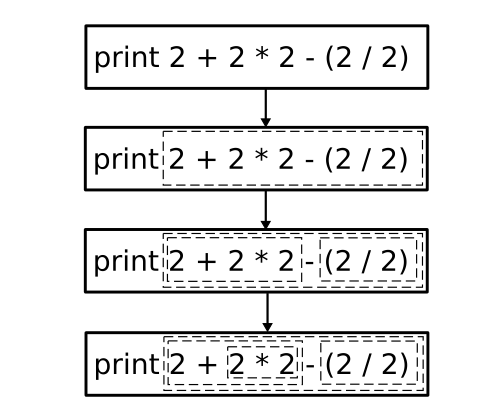
\includegraphics[width=300pt]{graphics/PrecedenceExample}
\caption{Operator Precedence Example}
\end{figure}

Every operator has a precedence level.  The interpreter finds operator with the lowest precedence, in this case in \SSCode{print} command, and then continues to simplify the remainder.  That is as deep as I will go into the inner workings of the expression evaluating engine, as long as you have an idea of how precedence works.  

Unary operators (like \SSCode{print}) have the lowest precedence.  Binary operators vary in their precedence level.  Here is a table you can refer to when you are unsure of precedence levels.  When two operators have equal precedence levels, they are executed from left to right.

\BeginSSTable{|c|c|}{h}
\textbf{Operator} & \textbf{Precedence} \\
\hline
\SSCode{( )} (Parenthesis) & $ \infty $ \\
\SSCode{:} (Scope Resolution) & 21 \\
\SSCode{[] -[] +[]} (List Access, Remove, and Append, respectively) & 20 \\
\SSCode{var list character player ...} (All object declaration operators) & 19 \\
\SSCode{not -} (Logical Not and Unary Negate\footnote{\emph{Not Minus!}}, respectively) & 19 \\
\SSCode{\^{}} (Exponentiation) & 18 \\
\SSCode{*} (Multiplication) & 17 \\
\SSCode{/} (Division) & 16 \\
\SSCode{.} (Concatenation) & 15 \\
\SSCode{+} (Addition) & 15 \\
\SSCode{-} (Subtraction) & 14 \\
\SSCode{,} (Listing Operator) & 13 \\
\emph{All other Unary Operators} & 12 \\
\SSCode{> <} (Greater-Than and Less-Than, receptively) & 11 \\
\SSCode{>= <=} (Greater-Than-or-Equal and Less-Than-or-Equal, respectively) & 10 \\
\SSCode{== !=} (Equal-To Not-Equal-To) & 9 \\
\SSCode{or} (Logical Or) & 8 \\
\SSCode{and} (Logical And) & 7 \\
\SSCode{\^{}=} (Exponent and Assign) & 6 \\
\SSCode{*=} (Multiply and Assign) & 5 \\
\SSCode{/=} (Divide and Assign) & 4 \\
\SSCode{.=} (Concatenate and Assign) & 4 \\
\SSCode{+=} (Add and Assign) & 3 \\
\SSCode{-=} (Subtract and Assign) & 2\\
\SSCode{=} (Assign) & 1 \\
\EndSSTable{Operation Precedence in \SSquared{}}

Remember, the expressions are evaluated from highest precedence level to lowest, and from left to right.  You don't have to memorize the precedence level of every operator and every condition.  In fact, given the experimental nature of this language, the possibly of minor changes occurring does exist.  If you are ever unsure about a situation, use parenthesis to clarify it.  Even if you are sure about a situation, it may confuse someone else using your code.  There is no real penalties for using parenthesis, and they can greatly clarify complicated expressions.

%
% Constrol Constructs
%
\chapter{Control Constructs}

\section{overview}

Control constructs are an essential part of any language.  They are a special part of a language that can perform loops and conditions.  Although the syntax is a little different than anything else in the language, the concept is pretty simple.  In the current version of \SSquared\ there are just three commands to worry about: \SSCode{if}, \SSCode{while}, and \SSCode{else}.

\section{if}

The syntax for if is pretty standard stuff, although it takes several forms.  Lets say that \SSCode{condition} is some expression that evaluates to a boolean result.  And that \SSCode{do\_something} and \SSCode{do\_something\_else} are other expression of some form.

\begin{SSCodeBox}
\scitea{} \\
\sciteg{//This is the first form}
\scitea{} \\
\scitee{if}
\scitea{ condition }
\scitee{then}
\scitea{ do\_something;} \\
\scitea{} \\
\sciteg{//This is the second form}
\scitea{} \\
\scitee{if}
\scitea{ condition} \\
\scitea{\{} \\
\scitea{\hspace*{4em}}
\sciteg{//The second form can execute more}
\scitea{} \\
\scitea{\hspace*{4em}}
\sciteg{//than one expression in its body.}
\scitea{} \\
\scitea{\hspace*{4em}do\_something;} \\
\scitea{\hspace*{4em}do\_something\_else;} \\
\scitea{\}}
\end{SSCodeBox}

The first form is very simple and English-like, but can only execute one expression if the condition is true.  The second for remedies this be allowing executing everything between the brackets if the condition is true.

It should be noted that the \SSCode{then} keyword and \SSCode{do} keyword are the exact same thing in \SSquared{}.  I included both named just to give the user the ability to make more grammatical looking expressions.




\section{while}

Loops in \SSquared\ are done using \SSCode{while}.  Which behavior is identical to that of \SSCode{if} with the exception that it will keep repeating the body until the condition become untrue.

\begin{SSCodeBox}
\scited{var}
\scitea{ i = }
\scitec{10}
\scitea{;} \\
\scitee{while}
\scitea{ i $>$= }
\scitec{0}
\scitel{} \\
\scitea{\{} \\
\scitea{\hspace*{4em}}
\scited{print}
\scitea{ i;} \\
\scitea{\hspace*{4em}}
\scited{print}
\scitea{ endl;} \\
\scitea{\hspace*{4em}i -= }
\scitec{1}
\scitea{;} \\
\scitea{\}}
\end{SSCodeBox}

That will keep printing \SSCode{i} and then subtracting one.  So it will print a countdown from 10 to 0.


\section{else}

The last control in \SSquared\ is \SSCode{else}.  The \SSCode{else} control has a couple variations, but always must be placed after an \SSCode{if} or \SSCode{while} control, and marks a section of code that gets executed if the body of the \SSCode{if} or \SSCode{while} is not executed.

\begin{SSCodeBox}
\scitee{if}
\scitea{ condition }
\scitee{then}
\scitea{ do\_something;} \\
\scitee{else}
\scitea{ }
\scitee{do}
\scitea{ something\_else;}
\end{SSCodeBox}

The \SSCode{do}, after the else is optional, since else statements have to condition and there is no need for separation.  Recall that \SSCode{do} is the same as \SSCode{then}.  They are both provided simply as syntactic sugar. 

Else statements can also take the brackets form.

\begin{SSCodeBox}
\scitee{if}
\scitea{ condition }
\scitee{then}
\scitea{ do\_something;} \\
\scitee{else}
\scitea{} \\
\scitea{\{} \\
\scitea{\hspace*{4em}do\_something\_entirely\_different;} \\
\scitea{\}} \\
\scitea{} \\
\sciteg{//or...}
\scitea{} \\
\scitea{} \\
\scitee{if}
\scitea{ condition} \\
\scitea{\{} \\
\scitea{\hspace*{4em}do\_something;} \\
\scitea{\}} \\
\scitee{else}
\scitea{} \\
\scitea{\{} \\
\scitea{\hspace*{4em}do\_something\_entirely\_different;} \\
\scitea{\}}
\end{SSCodeBox}

You can also put an else after a while, which is a bit unusual.  The body of the else will then be executed if the body of the while is never executed.


%
% Blocks
%
\chapter{Blocks}

\section{Overview}

Blocks are really the building ermm...blocks of \SSquared{}.  The have a dual role.  On one hand they are functions/subroutines/unary operators, and on the other hand they behave like lines of dialogue in a screenplay.  The sort of universal role of blocks is one of the central aspects of \SSquared{}.  If you've read this far into this document wondering where the actual storytelling aspect of \SSquared\ come into play, then thing swill start to make sense in the next few sections.

Blocks are declared simply by following an identifier with a beginning and ending bracket.

\begin{SSCodeBox}
\scitel{MyBlock}
\scitea{\{} \\
\scitea{\hspace*{4em}}
\sciteg{//This is the body of MyBlock.}
\scitea{} \\
\scitea{\}}
\end{SSCodeBox}

As you can see blocks simply delimits a chunk of code, and (optionally) assigns a name to it.  You can put really whatever you want between the brackets.  You can even declare other blocks within your block.  

\section{Transliteration}

Blocks like any other objects are automatically converted to variables.  When blocks are used in a variable context, their full name (their name plus all the scopes they belong to) is the result.  So if we used MyBlock in a variable context, it may give us \SSCode{:Test\_ssconv:MyBlock}, depending on the name of the file and such.

\section{Scopes}
\subsection{Concept}

Before we dive into blocks, we have to discuss the concept of scopes.  In the introduction I skimmed over the subjects, saying that scopes deal with ownership and who's allowed to touch who's stuff.  That's true, but there is a little more to it than that.

\begin{figure}[h]
\centering
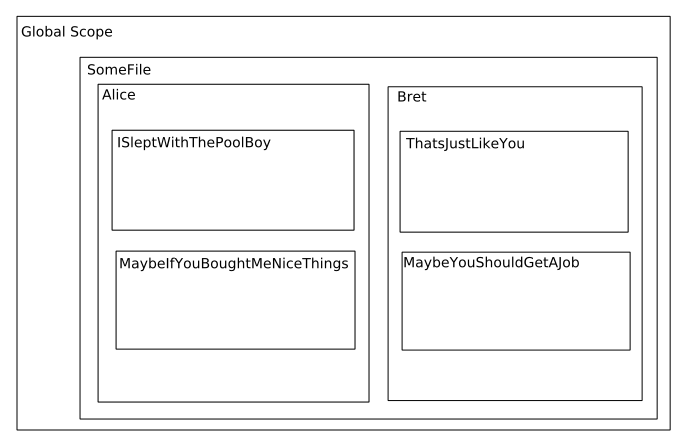
\includegraphics[width=\linewidth]{graphics/ScopeExample}
\caption{Scope Example}
\end{figure}

This is a more or less typical script file.  Each object has its own scope.  Every object that accessible with an identifier belongs to some other scope.  The is one root scope, a scope that contains every other scope.  In this example, the file being parsed (\SSCode{SomeFile}) resides in the global (root) scope.  Inside the file scope are two characters--Bret and Alice--who have a couple blocks each.

When interpreter searches for the object that a identifier refers to, it travels up the chain of ownership.  The interpreter will keep traveling up the chain looking in each scope until the first occurrence of the identifier.  So if you have two identifiers with the same name in separate scopes, you will get the one nearest down the chain, unless otherwise specified.

One way to visualize scopes is to imagine that each scope is a room with wall made out of two way mirrors\footnote{Dropping acid before hand can help.}.  Anyone can see out of the rooms, but no one can see in.  For example, from inside Bret's scope, you can see the Alice scope, but you can't see what is in the Alice scope.  You can even see the Alice scope from inside one of the blocks in the Bret scope.

So if we want to access Alice from within a block that belongs to Bret, we can just call her by name.

\begin{SSCodeBox}
\scitel{Bret: ThatsJustLikeYou}
\scitea{\{} \\
\scitea{\hspace*{4em}}
\scited{out}
\scitea{ =} \\
\scitea{\hspace*{4em}}
\sciteb{"That's just like you, "}
\scitea{ . Alice . }
\sciteb{"."}
\scitea{;} \\
\scitea{\}}
\end{SSCodeBox}

Alice exists outside of the scope of the block and therefore can be accessed without any kind of scope resolution.  (Take notice that this is kind of a silly example.  Using the Alice identifier in that way is pointless, and won't even work how the example implies.)

\subsection{Scope Resolution}

If we want to refer to some block that belongs to Alice, we need to use the scope resolution operator (\SSCode{:}).  We may be able to see Alice from inside Bret, but we cant see into Alice.  The scope resolution operator tells the interpreter to search in a specific scope for an identifier.

Because the last example doesn't really work the way we want.  Lets use the \SSCode{name} magic variable that belongs to Alice.

\begin{SSCodeBox}
\scitel{Bret: ThatsJustLikeYou}
\scitea{\{} \\
\scitea{\hspace*{4em}}
\scited{out}
\scitea{ =} \\
\scitea{\hspace*{4em}}
\sciteb{"That's just like you, "}
\scitea{ . Alice:name . }
\sciteb{"."}
\scitea{;} \\
\scitea{\}}
\end{SSCodeBox}

Here the scope resolution operator (the colon) is used after Alice's name to specify what scope to search in for the identifier name.  Scope resolution operators can be chained together like any other binary operator.

\begin{SSCodeBox}
\scited{print}
\scitea{ Alice:name:name;}
\end{SSCodeBox}

That will just print ``name'', which is pointless but mildly amusing if you're up at 3 A.M. and heavily intoxicated.

\subsection{Characters}

Characters a represented in \SSquared\ simply by a scope.  Characters are declared just like variable or lists, but using the \SSCode{character} keyword.

\begin{SSCodeBox}
\scited{character}
\scitea{ Francis;}
\end{SSCodeBox}

Normal naming rules apply. They are unlike blocks or variables in that they have no special attributes.  They are simply empty scopes.  That all there is to it.

\subsection{Importing}

\SSquared\ gives you the ability to import scopes into each other.  If were to continue with the (terrible) two-way-mirror metaphor, importing scopes is like opening a viewport into another scope.

\begin{figure}[h]
\centering
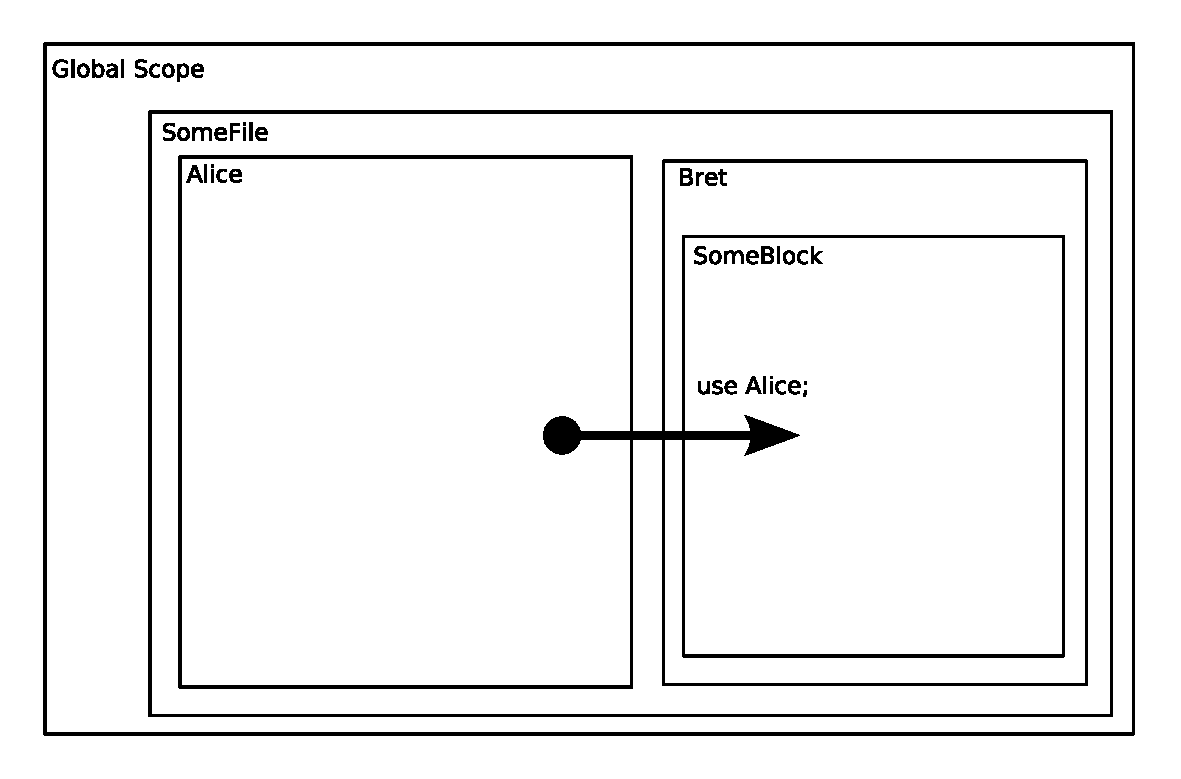
\includegraphics[width=\linewidth]{graphics/ScopeExample2}
\caption{Scope Example}
\end{figure}

If you take a look at Figure 5.2 you can (maybe) see in the figure, the syntax for importing scope is fairly straightforward.

\begin{SSCodeBox}
\scited{use}
\scitea{ Alice;}
\end{SSCodeBox}

I'm not sure if Alice would appreciate Bret using her, but what she doesn't know won't hurt her.  This imports the Alice scope into whatever the current scope happens to be.  Now if the interpreter does not find an identifier by searching down the ownership chain, it will check the Alice scope.

\subsection{Importing Files}

The other important task that the \SSCode{use} keyword performs is importing files.  The same syntax is used, but with a file name instead of an scope name.

\begin{SSCodeBox}
\scited{use}
\scitea{ }
\sciteb{"MyOtherFile.ssconv"}
\scitea{;}
\end{SSCodeBox}

Each file that gets loaded has its own scope.  When you import a file, if the file is not already open, the interpreter will open it and parse the file and then import the newly created scope.  If the file has already been opened, its scope will be imported.

When a file gets loaded for the first time, the interpreter executes anything on the top level.  That is, it executes any code that isn't in blocks.  When it comes across a block, it declares it, and then skips over the body.  So you can certainly reference a block at the end of a file from within a block at the beginning.  But anything you declared inside a block won't exist until that block gets executed in some form.

The names of the file scopes are mangled in a way to conform to object naming rules.  Any illegal characters (such as periods) are replaced by underscores when the scope is made.  So \SSCode{Foo.ssconv} become \SSCode{Foo\_ssconv}.

\section{Blocks as Lines in a Script}

The original and central intent of blocks is to behave lines of dialogue.  Inside each block is a built variable called \SSCode{out}.  When the interpreter reads the blocks in dialogue mode, have the owner of the block say whatever is in the out strings.

\begin{SSCodeBox}
\scited{character}
\scitea{ Ishmael;} \\
\scitea{} \\
\scitel{Ishmael:}
\scitea{\{} \\
\scited{out}
\scitea{ =} \\
\sciteb{"But so have I seen little Miriam and Martha, laughing-eyed elves, heedlessly gambol around their old sire; sporting with the circle of singed locks which grew on the marge of that burnt-out crater of his brain."}
\scitea{;} \\
\scitea{\}}
\end{SSCodeBox}

This is an example of an unnamed block.  It simply uses the scope resolution operator with nothing after it.  The interpreter just creates the new block with no name in the Ishmael scope.  When this block gets ``said'', whatever is in the out string (in this case part of a very moving description of Captain Ahab) said.  What I mean by ``said'' varies depending on how the game using \SSquared\ decides to implement it.  If you are simply using the command line interface, then it will print the characters name and then the line in pretty colors.

\subsection{Out Strings}
Out(put) strings are a shorthand way of assigning literals to the \SSCode{out} variable.  They resemble normal strings, but they use backticks (\`{}) as the quotation marks.  This tells the interpreter to append that string to the out variable. 

\begin{SSCodeBox}
\scitel{Doc:}
\scitea{\{} \\
\scitem{`One point twenty one GIGAWATTS!\`{}}
\scitea{;} \\
\scitea{\}}
\end{SSCodeBox}

This is the exact equivalent of just assigning it to the out variable.  These strings also stack with other out strings strings.

\subsection{next}

The standard behavior of the interpreter when it loads a new file is the say he first block and say the next block down the file and continue to proceed like that.  In other words, it just works like reading a linear, deterministic script.  One character says one thing, and then another character says something else.

To override this behavior you must set \SSCode{next}, which is a list that every block has built-in.  The \SSCode{next} list gets set with the names of one or more blocks, which tells the interpreter how to proceed.  If there is only one block name, it will jump straight to that block after it finishes saying the current block.  If there are more however, the player will be presented with a choice and must choose the next thing that is said.  This is a pretty simple way to replicate branching dialogue as seen in many computer RPG's.  

\begin{SSCodeBox}
\scited{character}
\scitea{ Jack;} \\
\scited{character}
\scitea{ Jill;} \\
\scitea{} \\
\scitel{Jack:}
\scitea{\{} \\
\scitem{`Hey, Jill`}
\scitea{;} \\
\scitea{\}} \\
\scitea{} \\
\scitel{Jill:}
\scitea{\{} \\
\scitem{`Hi, Jack`}
\scitea{;} \\
\scitea{\}} \\
\scitea{} \\
\scitel{Jack:}
\scitea{\{} \\
\scitem{`So what's new?`}
\scitea{;} \\
\scitea{} \\
\scited{next}
\scitea{=} \\
\scitea{Jill: NotMuch,} \\
\scitea{Jill: TheUsual,} \\
\scitea{Jill: IHaveCancer;} \\
\scitea{\}} \\
\scitea{} \\
\sciteg{//...}
\end{SSCodeBox}

This script will be executed linearly until it gets to last block in which the player is presented with a choice.  This also assumes that those block exists somewhere, otherwise you will get an error.  How the player is presented with the choice is another detail that is left up to the interface.  From the command line you will just input a number corresponding to the choice.

You may also set the next list to \SSCode{end}, which instruct it the end the conversation.  Be sure to remember to do this.  Otherwise it will continue executing blocks.

\subsection{Doc Strings}
Doc(ument) Strings are a very recent addition.  When blocks a block is being used as dialogue, it will be the string presented for that block when the player must make choice between several blocks.  Without the doc string, the the choice presented will just be the full name of the block, which is not really desirable.

Doc strings have somewhat unusual syntax.  They are strings like any others, but they use single quotes (\').  Furthermore, the \emph{must} be placed immediately after the left bracket (\SSCode{\{}) in block declarations.  You should also not put a semicolon after the string as you do with out strings.  This syntax is a little confusing at first.  It helps to think of doc strings as extensions of the block declaration rather than an expression.  That is how the interpreter treats them.

In similar fashion to out strings begin assigned to \SSCode{out}, doc strings are assigned to \SSCode{doc}, which is a built-in member of every block.

Let's add onto the last example using doc strings to write the responses.

\begin{SSCodeBox}
\sciteg{//...}
\scitea{} \\
\scitea{} \\
\scitel{Jill: NotMuch}
\scitea{\{} \\
\scitea{\hspace*{4em}}
\sciten{'Not much.'}
\scitea{} \\
\scitem{`Not much, Jack.`}
\scitea{;} \\
\scitea{} \\
\scitea{\hspace*{4em}}
\scited{next}
\scitea{ = }
\scited{end}
\scitea{;} \\
\scitea{\}} \\
\scitea{} \\
\scitea{} \\
\scitel{Jill: TheUsual}
\scitea{\{} \\
\scitea{\hspace*{4em}}
\sciten{'Just the usual.'}
\scitea{} \\
\scitem{`Oh, you know.{\hspace*{1em}} The usual.`}
\scitea{;} \\
\scitea{\hspace*{4em}} \\
\scitea{\hspace*{4em}}
\scited{next}
\scitea{=}
\scited{end}
\scitea{;} \\
\scitea{\}} \\
\scitea{} \\
\scitel{Jill: IHaveCancer}
\scitea{\{} \\
\scitea{\hspace*{4em}}
\sciten{'I have cancer.'}
\scitea{} \\
\scitem{`I have cancer and only have two weeks to live.{\hspace*{1em}} How are doing?\`{}}
\scitea{;} \\
\scitea{} \\
\scitea{\hspace*{4em}}
\scited{next}
\scitea{=}
\scited{end}
\scitea{;} \\
\scitea{\}}
\end{SSCodeBox}

When the entire script gets executed, the player will be presented with three choices: ``Not much.'', ``Just the usual.'', and ``I have cancer.''.  Remember: single quotes, directly after the opening bracket, and no semicolon.  These strings should follow normal string rules.  They will stack with each other and backslashes should behave how they do in normal strings as well.

\section{Blocks as Functions}

\subsection{Overview}

Blocks also second as user-definable functions.  \SSquared\ was designed in a way that writing dialogue blocks is remarkably similar to writing function blocks.  All functions in \SSquared\ take a list as their argument, and return a variable.

The input list is called \SSCode{in}, which I thought was an appropriate counter to \SSCode{out}.  A block can take arguments from the \SSCode{in} list and then assign to the \SSCode{out} variable.  When the block finishes executing the out variable will be return value.  Here is an example of block that calculates the factorial of a given value.

\begin{SSCodeBox}
\scitel{fact}
\scitea{\{} \\
\scitea{\hspace*{4em}}
\scited{out}
\scitea{ = }
\scitec{1}
\scitea{;} \\
\scitea{\hspace*{4em}} \\
\scitea{\hspace*{4em}}
\scitee{while}
\scitea{( in[}
\scitec{0}
\scitea{] $>$ }
\scitec{1}
\scitea{ )} \\
\scitel{\hspace*{4em}}
\scitea{\{} \\
\scitea{\hspace*{4em}\hspace*{4em}}
\scited{out}
\scitea{ *= in[}
\scitec{0}
\scitea{];} \\
\scitea{\hspace*{4em}\hspace*{4em}in[}
\scitec{0}
\scitea{] -= }
\scitec{1}
\scitea{;} \\
\scitea{\hspace*{4em}\}} \\
\scitea{} \\
\scitea{\hspace*{4em}}
\scited{next}
\scitea{=}
\scited{end}
\scitea{;} \\
\scitea{\}}
\end{SSCodeBox}

The first element of \SSCode{in} is used, and the result is assigned to the \SSCode{out} variable.  It is safe to use the \SSCode{in} variable this way, even if it's empty.  The first element will just be created with the default initial value.   The \SSCode{next=end} is necessary so the interpreter will not try to execute blocks following it.  This function is simply called as any other unary operator.

\begin{SSCodeBox}
\scited{print}
\scitea{ fact }
\scitec{5}
\scitea{;}
\end{SSCodeBox}

This passes \SSCode{5} in the fact's \SSCode{in} list, and when fact finishes executing, the expression evaluates to the value in fact's \SSCode{out}.

\subsection{return}

A sometimes simpler and more conventional handle the return value is to use the \SSCode{return} function.  The \SSCode{return} function will set the out variable and then immediately end execution of the block.  This can make some function blocks simpler to read and write.

\begin{SSCodeBox}
\scitel{AddTwo}
\scitea{\{} \\
\scitea{\hspace*{4em}}
\scited{return}
\scitea{ in[}
\scitec{0}
\scitea{] + }
\scitec{2}
\scitea{;} \\
\scitea{\}}
\end{SSCodeBox}

\subsection{Doc Strings}

Doc strings also serve a purpose with function blocks.  Setting the doc string can give the user of your function a better understanding of what it does and how to use it.  If we were to write our AddTwo function with a doc string, it may look like this.

\begin{SSCodeBox}
\scitel{AddTwo}
\scitea{\{} \\
\sciten{'Takes one argument and returns the argument plus two.'}
\scitea{} \\
\scitea{\hspace*{4em}}
\scited{out}
\scitea{ in[}
\scitec{0}
\scitea{] + }
\scitec{2}
\scitea{;} \\
\scitea{\}}
\end{SSCodeBox}

When someone wants to know how to use the AddTwo function, they can simply have the interpreter print \SSCode{AddTwo:doc}.



%TODO: Everything under this section.

%
% Other Topics
%
\chapter{Miscellaneous Topics}

\section{LangOpts}

Language Options or LangOpts is a recent addition to \SSquared\ and part of a longer term plan I have to give the user further ability to change how the language works from within the language.  On the advantages of an interpreted language is the it allows for this.  Right now LangOpts has only a couple of options, but it's a start.  All of members of LangOpts are magic variables, and I would not recommend modifying them and are considered advanced options that you typically will not have to modify.

\subsection{default\_precision}

The default\_precision magic variable gives you control over the default precision of newly created variables.  The precision is measured in bits.  The current default (which is guarantees to stay the same in future versions) is 256, which is usually higher than you need.  However, if you want to perform some really insane calculations, default\_precision may be of some use to you.

\subsection{rounding\_mode}

This magic variable changes the method by which variables are rounded in math operations.  The default is to round to the nearest value, with half way values rounded up.  This is the way rounding is typically done, but MPFR library gives you some options which I decided to pass along to \SSquared\ users.  The other options are to round towards zero (rounding up if negative, rounding down if positive), rounding towards infinity (always rounding up), and rounding towards negative infinity (always rounding down).

Currently, this magic variable is a little user unfriendly and you have to set it to a number.  The numbers corresponding to the mode are:

\BeginSSTable{|c|c|}{h}
\textbf{Mode} & \textbf{Code} \\
\hline
Towards Nearest & 0 \\
Towards Zero & 1 \\
Up & 2 \\
Down & 3 \\
\EndSSTable{Rounding Modes}



\subsection{max\_digit\_output}

By default, when numbers get automatically transformed into strings, they will spit out every digit in the number.  Setting max\_digit\_output to some number will force the interpreter to limit the number of digits outputted.  The default value is 0, which instructs the interpreter to output every digit.

\subsection{number\_base}

You are able to change he base of numbers by settings number\_base to something other than 10.   Be aware, however, number\_base will \emph{always} report its value as 10.  For example, if you set the base to 2, and then print number\_base it will print 2, in base 2, which is of course 10.  So you must be careful when using this.  To go from base 2, back to base 10, you must set number\_base to 110 (10 in binary).  If that sounds confusing, you better not mess with this.  

In the current version of the interpreter, this value is highly experimental and probably doesn't work correctly yet.

\subsection{use\_strict\_lists}

As mentioned in the list chapter, the normal behavior of \SSquared\ is to spring new list elements into existence when you call on them.  This can be changed so you must explicitly create each element.  To do so, simply set use\_strict\_lists to true.

\subsection{verbose}

The interpreter is capable of spitting out a lot of debugging information that you normally don't care about, but can be useful for debugging the interpreter.  Setting verbose to true gives a convenient way to turn this information on or off for only certain sections.  Turning it on is the equivalent of passing the ``--ungodly-verbose'' flag on the command line.


%
% SLib
%

\chapter{SLib: The \SSquared\ Standard Library}

\section{Introduction to the Standard Library}
Larry Wall, who invented another language called Perl, wrote that the ``the three chief virtues of a programmer are Laziness, Impatience and Hubris.''  I consider laziness one of the most important.  Why bother implementing something when its already when there is already a good implementation available.

Here's a joke I heard:  An engineer, a physicist, and a mathematician were staying at the same hotel.  The engineer left her curling iron on which ignited a towel.  She quickly threw the towel in the sink and turned the water on.  Merely a few hours later, the physicist who was staying down the hall had his toaster burst into flames.  He pondered this for a moment and threw a blanket over the toaster cutting off the oxygen supply to the fire and quickly putting it out.  The mathematician who smelled the smoke and came to help saw that the fire was already out so he returned to his room.  As luck would have it, in his panic he had thrown his lit cigar into the trash, which he discovered had ignited.  When he saw this he was initially startled, but then he thought about it, and exclaimed, ``Ah!  A solution exists.''  And then he went to bed.

S-Lib is a collection of solutions for everyday chores.  While \SSquared is certainly powerful for you to write your own code to do these chores, S-Lib has two advantages.  The first advantage is speed.  The S-Lib functions are all written in C++ (as is the rest of the interpreter), which is a compiled language which inherently will have less overhead than interpreted languages (like \SSquared{}).  The second advantage is rather simple: its already there.  You don't have to write anything, just look up the function and use it.

All the S-Lib code is in modules which are in their own scopes.  You can import these scopes just like you can any scope using the ``use'' operator (e.g.. \SSCode{use SSMath}).  Or you can just access them through their scopes.  Some of the more common S-Lib scopes are already imported by default.

In the following sections, all the S-Lib operators are listed out with their inputs and outputs and any side-effects.

\section{SSCommon}
The SSCommon scope is imported by default and contains many\footnote{Very few right now. :(} operators that are used, well, commonly.

\SSFunctionDesc{print}
{One argument, any lists gets squashed into one variable.}
{Prints the argument to the screen in one way or another, depending on the implementation.}
{The printed argument.}

\section{SSList}
The SSList scope contains many useful operators for use with lists.  It is also imported by default.

\SSFunctionDesc{pickone}
{Any list.}
{Randomly selects an element from the list and returns it.}
{Uses a Mersenne Twister pseudo-rng.}

\SSFunctionDesc{reverse}
{Any list.}
{Creates a new list with all the elements of the the given list in reverse order and returns it.}
{}

\SSFunctionDesc{sort}
{Any list.}
{Returns a sorted version of the original list. }
{It sorts alphabetically using quicksort.  Numbers and symbols come before letters.  Numbers are sorted alphabetically meaning that they are not necessarily in order of size.}

\section{SSMath}
The SSMath scope is not imported by default.  It contains many useful mathematical operations, since many of these would be difficult and slow to implement in \SSquared{}


\SSFunctionDesc{sqrt}
{Any variable.}
{Returns the \emph{square root} of the given variable.}{}

\SSFunctionDesc{abs}{Any variable.}
{Returns the \emph{absolute value} of the given variable.}{}

\SSFunctionDesc{mean}
{Any List.}
{Returns the mean (average) value of the list.}{}

\SSFunctionDesc{sin}{Any variable.}{Returns the sine of the variable.}{Input is in radians.}

\SSFunctionDesc{cos}{Any variable.}{Returns the \emph{cosine} of the variable.}{Input is in Radians.}

\SSFunctionDesc{tan}{Any variable.}{Returns the \emph{tangent} of the variable.}{Input is in radians.}

\SSFunctionDesc{asin}{Any variable.}{Returns the \emph{arc-sine} (inverse sine) of the variable.}{Output is in radians.}

\SSFunctionDesc{acos}{Any variable.}{Returns the \emph{arc-cosine} (inverse cosine) of the variable.}{Output is in radians.}

\SSFunctionDesc{atan}{Any variable.}{Returns the \emph{arc-tangent} (inverse tangent) of the variable.}{Output is in radians.}

\SSFunctionDesc{max}{Any list.}{Returns the largest number in the list.}{Strings are treated as zero.}

\SSFunctionDesc{min}{Any list.}{Returns the smallest number in the list.}{Strings are treated as zero.}

\SSFunctionDesc{int}{Any variable.}{Returns the variable rounded to the nearest integer.}{Half-way cases (eg. 0.5) are rounded up.}

\SSFunctionDesc{floor}{Any variable.}{Returns the variable rounded to the next lowest integer.}{}

\SSVariableDesc{pi}{Evaluates to the $\pi$ (pi) constant.}{The precision variable functions just like in any other variable.}

\SSVariableDesc{e}{Evaluate to the e (Euler) constant.}{The precision variable functions just like in any other variable.}

\section{SSTime}
The SSTime scope contains functions and magic variables for working with dates and times.  The outputs of these can be somewhat dependent on the operating system.

\SSVariableDesc{date}{Evaluates to the current date of the system running the interpreter.}{The output will be in DD/MM/YYYY (or DDMMYYYY in a number context) format, but it may vary slightly from system to system.}

\SSVariableDesc{time}{Evaluates the current time on the system running the interpreter.}{Time is given in (H)H:MM:SS AM/PM format in string context, and in a number context HHMMSS.}

\SSVariableDesc{timezone}{Gives the current time-zone of the system running the interpreter.}{Output format will vary from system to system.  Some abbreviate, some do not.}

\SSVariableDesc{elapsed\_seconds}{Returns the number of seconds passed since the interpreter began running.}{This is useful for checking how much time has passed between two events.  Just save the time at the first event to a variable.  Later, subtract that variable from the ElapsedSecond at the second event.  Note that the precision and maximum value of this varies among operating systems and computers.  Usually it can go up to at least several hundred hours and have a precision in the milliseconds.}
